\chapter{Sources of loss}
\label{chp:loss}

The number of KIDs that can be multiplexed depends on the bandwidth needed by each resonator and the total bandwidth of the readout electronics.
The resonator linewidth -- that is, the full-width, half-maximum bandwidth -- is
$b_\resonator = \loss_\resonator \freadout_\resonator$.
To avoid resonance collisions and minimize electronic crosstalk one might design for adjacent resonance frequencies to be separated by at least 5 times $b_\resonator$.
For reasonable multiplexing, one might require
$\loss_\resonator = \loss_\internal + \loss_\coupling < \num{e-4}$,
corresponding to
$\qf_\resonator > \num{e4}$.
If the resonators are designed so that $\loss_\coupling \approx \loss_\internal$ under the expected optical load, this gives $\loss_\internal \lesssim \num{5e-5}$.
The device sensitivity is improved when the quasiparticle loss dominates the total internal loss so that $\qpfraction$ approaches 1.

The total internal loss is the sum of all the relevant loss terms:
\begin{equation}
\loss_\internal
  =
  \loss_\quasiparticle +
  \loss_\substrate +
  \loss_\tls +
  \loss_\mathrm{nf} +
  \loss_\vortex +
  \cdots,
\end{equation}
where the terms shown here correspond respectively to quasiparticle loss (Section~\ref{sec:theory.response}), loss due to the bulk dielectric substrate and due to two-level systems on nearby surfaces (Section~\ref{sec:loss.dielectrics}), 
loss caused by near-field coupling to normal metal (Section~\ref{sec:loss.near-field}),
and loss due to magnetic flux vortices (Section~\ref{sec:loss.vortex}).
Another possible source of loss is radiation, which may propagate either into the substrate or into free space~\autocite{Sage2011JAP,Zmuidzinas2012ARCMP}.
From the above design requirements, we see that the sum of all non-quasiparticle loss terms should satisfy
$\loss_\internal - \loss_\quasiparticle \ll \num{5e-5}$.


\section{Dielectrics}
\label{sec:loss.dielectrics}

\todo[inline]{Create dielectric constant notation.}
\todo[inline]{Use expressions from Jackson or Pozar to relate the energy stored and lost.}
\todo[inline]{Try to convert the energy storage and loss into a 1D problem.}
\todo[inline]{How are electric and magnetic energies defined when kinetic inductance is significant?}
\todo[inline]{Explain how energy is lost in a bulk dielectric.}
\todo[inline]{Discuss recent TLS papers.}

KIDs are typically fabricated on single-crystal dielectrics with very low loss, such as sapphire and intrinsic silicon.
With careful fabrication and shielding, aluminum co-planar waveguide resonators on sapphire have achieved $\loss_\internal \approx \num{e-6}$ at single-photon readout levels, and as low as $\loss_\internal \approx \num{e-7}$ at higher readout power, which suppresses the dielectric loss~\autocite{Megrant2012APL}.
With one exception, all of the resonators discussed in this thesis are fabricated on high-resistivity, float-zone silicon substrates.
Thus, we can neglect the loss due to the bulk substrate except possibly under dark conditions, where the quasiparticle loss is extremely low.
(The exception to the above is the prototype 23-pixel multichroic KID array discussed in Section~\ref{sec:multichroic.mkidarray02}, which is fabricated on a silicon-on-insulator wafer that contains a silicon oxide layer and a lower-resistivity thick handling wafer.)

Two-level systems (TLS) that occur in amorphous dielectrics at interfaces, such as surface oxides, are a more significant source of loss in superconducting resonators~\autocite{Gao2007APL, OConnell2008APL,Gao2008aAPL,Gao2008bAPL,Wang2009APL,Wenner2011APL}.
The loss due to TLS is given by
\begin{equation}
\loss_\tls
  =
  \loss_{\tls, 0} \frac{\tanh \left( \planck \freadout / \kb \temperature \right)}{\left[1 + (\power_\internal / \power_*)^{\beta / 2} \right]^{1/2}}
\end{equation}
where $\loss_{\tls, 0}$ is the low-power loss, $\power_\internal$ is the power flow into the resonator, $\power_*$ is a critical power that depends on the TLS physics, and the exponent $\beta \approx 1.6 - 2$ depends on the resonator geometry~\autocite{Wang2009APL}.
The critical power is much less than the power levels typically used with KIDs, so we expect
$\loss_\tls \propto \power_\readout^{-0.5}$
or a slightly weaker dependence~\autocite{Zmuidzinas2012ARCMP}.

The loss contributed by dielectrics in a given region depends on the fraction of electric field energy in that region.
Using the definition of the quality factor (or its inverse) we can write
\begin{equation}
\loss_\mathrm{dielectric}
  =
  \sum_i
  \loss_i
  =
  \sum_i
  \alpha_i \tan \delta_i,
\end{equation}
where the index $i$ refers to different dielectrics that occupy different regions, the participation ratio $\alpha_i$ equals the fraction of total electric energy in the volume occupied by the $i$th dielectric, and $\tan \delta_i$ is the intrinsic loss tangent for that dielectric~\autocite{OConnell2008APL}.
Assuming that the losses are small enough not to perturb the field configuration, one can extract the participation ratio for a dielectric using electromagnetic simulations that use several different loss tangents for that dielectric, and fitting the results.

\todo[inline]{TLS fractional frequency shift}


\section{Near-field coupling}
\label{sec:loss.near-field}

\todo[inline]{Discuss radiation into free space: slot antenna.}
\todo[inline]{Discuss radiation into the substrate caused by quasi-TEM phase velocity being faster than in bulk.}

In an early generation of aluminum lumped-element resonators on intrinsic silicon, we measured internal loss $\loss_\internal \approx \num{2.5e-5} = 1 / \num{40000}$, which was significantly lower than expected~\autocite{McCarrick2014RSI}.
At several millimeters on a side, these devices were much larger than the substrate thickness of about \SI{0.5}{mm}.
(This large area was required to produce resonance frequencies around \SI{100}{MHz}.)
These devices were tested in packages machined from oxygen-free, high conductivity copper with gold plating.
The model we developed was that the resonator fields were still sufficiently large at the surface of the package, on the opposite side of the substrate, to produce dissipation due to the interaction with the relatively lossy normal metal.

To test this idea, we fabricated subsequent packages from aluminum alloys (mostly 6061-T6 and QC-10) that we measured to superconduct near the bulk aluminum transition temperature of \SI{1.2}{K}.
Lumped-element resonators tested in these packages had much lower internal loss, typically
$\num{e-6} < \loss_\internal < \num{e-5}$, indicating that switching to aluminum had greatly reduced the dissipation.
Additional evidence for this theory came from later observations that all-niobium lumped element resonators with large capacitors responded to temperature changes well below \SI{1}{K}, qualitatively as expected for aluminum, while co-planar waveguide (CPW) resonators fabricated on the same wafer did not respond to such temperature changes.
This is consistent with the CPW fields being more strongly confined, due to the ground plane, and thus interacting less with the material beyond the substrate. 
\textcite{Goetz2016JAP} showed that this source of loss may also occur in CPW resonators if the substrate is sufficiently thin and the material on the opposite side is sufficiently lossy.

Quantifying the loss in the early experiments was complicated by the fact that the aluminum may have also improved the magnetic shielding around the detectors.
We did not perform additional experiments to conclusively attribute the excess loss to near-field coupling instead of the magnetic flux vortices discussed in the following section.
Superconducting aluminum is expected to have much lower thermal conductivity than copper, due to the absence of an electronic contribution, but we have seen no evidence that the thermal conductivity is insufficient.


\section{Magnetic flux vortices}
\label{sec:loss.vortex}

This section describes an experiment we performed in order to better understand anomalous loss in lumped-element resonators.
This research was published as \fullcite{Flanigan2016bAPL}.

\begin{figure}[tbp]
\centering
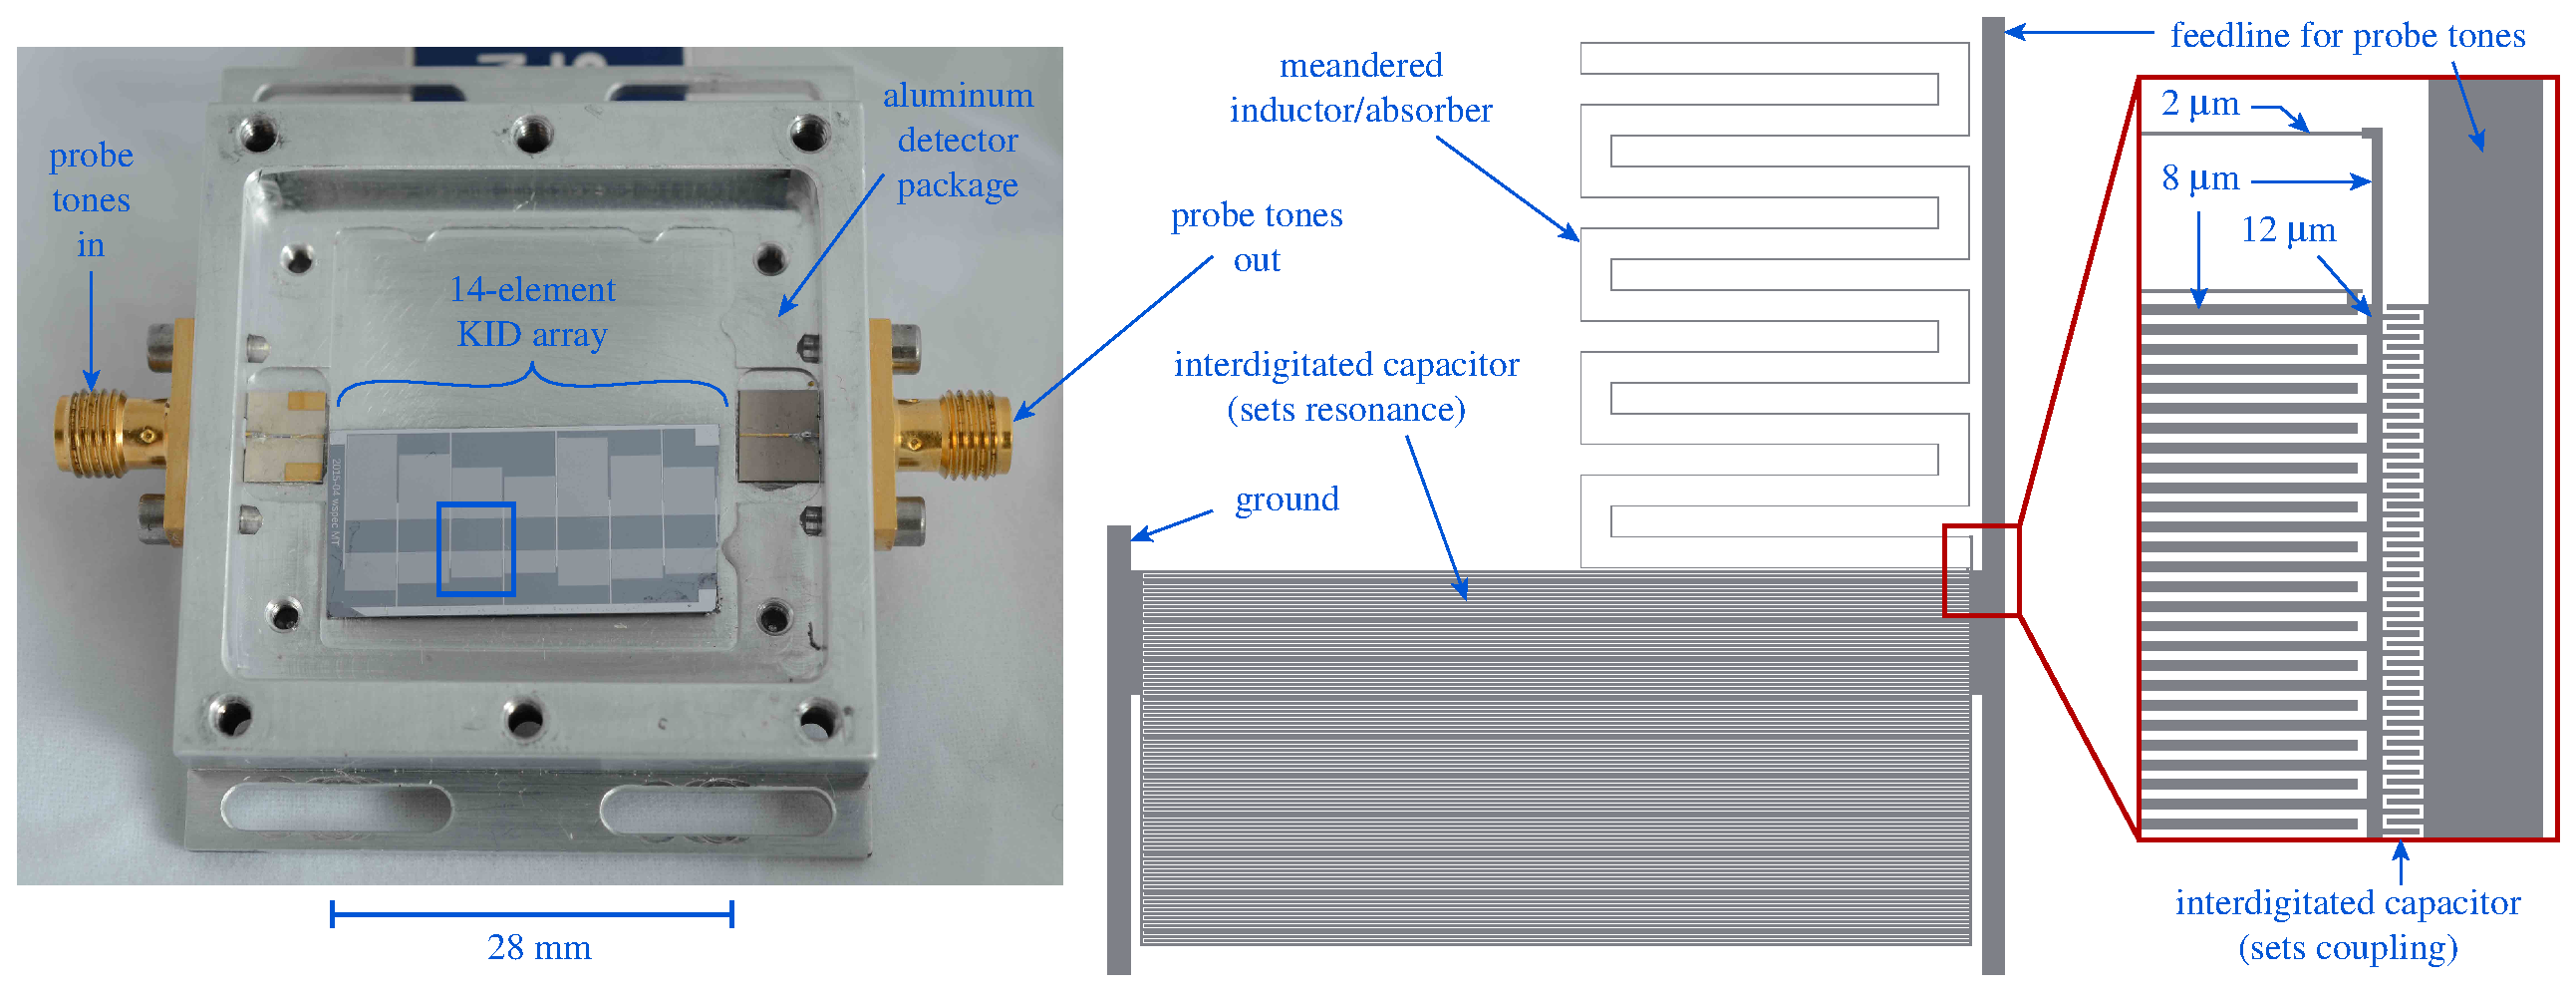
\includegraphics[width=\textwidth]{loss/experiment.eps}
\caption
[Photographs and drawings of the magnetic flux vortex experiment.]
{Photographs and drawings of the magnetic flux vortex experiment.
\textbf{Left:}
A photograph of the detector module tested in this study.
The package lid is removed and the KID array is visible.
Metal clips, not shown here, are used to hold the KID array in place.
\textbf{Center:}
A scale drawing of the lumped-element KID in the blue box on the left.
\textbf{Right:}
Detail of the center panel, showing all of the trace widths used in the resonator.
Our hypothesis is that the ambient magnetic field in the experimental volume was sufficiently strong to create vortices in the widest (\SI{12}{\micro m}) trace, causing unexpectedly high loss.}
\label{fig:loss.experiment}
\end{figure}

\subsection{Introduction}

The suitability of KIDs as a detector technology for photometry depends in part on the fact that they can exhibit high resonator quality factors $\qf_\resonator$.
By tuning each resonator to a unique frequency and taking advantage of the narrow bandwidth corresponding to high $\qf_\resonator$, hundreds or thousands of KIDs may be read out on the same feed line using frequency division multiplexing.
To maintain excellent noise performance and multiplexing capability, it is desirable for the internal loss to be dominated by quasiparticles.

Before incorporating magnetic shielding in the cryostat used to test detectors, we sometimes observed internal quality factors significantly lower than expected.
The packages we use to test KIDs are made from aluminum, a type-I superconductor, which should expel external magnetic fields when superconducting and thus could function as a magnetic shield.
Indeed, after the system is cooled well below the bulk aluminum critical temperature of \SI{1.2}{K}, the KIDs do not detectably respond to externally applied magnetic fields, regardless of their internal quality factors.
However, thin films of type-I superconductors permit magnetic flux entry in the form of vortices~\autocite{Tinkham1963PR,Dolan1974aJLTP}.
These vortices produce loss in thin-film superconducting resonators~\autocite{Song2009PRB,Wang2009APL,Mazin2010APL,Bothner2011APL,Bothner2012PRB,deGraaf2012JAP,Nsanzineza2014PRL,Chiaro2016SUST} because an alternating current in a thin-film trace produces an oscillating Lorentz force on a vortex, and the vortex motion is dissipative~\autocite{Song2009PRB}.

We developed the following hypothesis to explain the excess loss: since the thin film used in the KID has a critical temperature $\tc = \SI{1.4}{K}$, and thus transitions before the package when the system is cooled, vortices formed in the un-shielded film become trapped there and persist when the package becomes superconducting as the system is cooled far below $\tc$.
The presence of vortices at the KID operating temperature (about \SI{150}{mK}) would depend on the field present when the aluminum film transitions.
We tested this hypothesis by varying the strength of the ambient field at \SI{1.4}{K} and measuring $\qf_\internal$ at the KID operating temperature.


\subsection{Experiment}

The resonators used in this study are lumped-element kinetic inductance detectors~\autocite{Doyle2010SPIE} lithographically patterned from a \SI{20}{nm} thick aluminum film on a \SI{500}{\micro m} thick high-resistivity, float-zone silicon substrate.
They were designed for astrophysical measurements at millimeter wavelengths.
The detectors tested in this study were not optically illuminated and were instead mounted inside a light-tight aluminum package with copper tape covering the seam to prevent light leaks.
The package was machined from QC-10, an aluminum alloy for which we have measured a critical temperature near that of bulk aluminum (\SI{1.2}{K}).
The left panel of Figure~\ref{fig:loss.experiment} is a photograph of the KID array in the package.
Fourteen resonators were patterned in this array.
For this study we focused on just three of these resonators, with resonance frequencies $\freadout_\resonator$ of \SIlist{78;116;161}{MHz}.
The center and right panels of Figure~\ref{fig:loss.experiment} are drawings of one resonator that show the various trace widths used in different regions.
The width of the traces is important here because magnetic flux vortices will form at lower field magnitudes in wider traces.
Figure~\ref{fig:starcryo_cryostat_with_optics_box} is a photograph of the cryostat used in this experiment.
Inside the cryostat, the package was mounted to a gold-plated copper plate that is thermally connected to the cold stage of an adiabatic demagnetization refrigerator (ADR) backed by a helium pulse tube cooler.

The ambient magnetic field of the room in the region of the package was measured to be downward to within \SI{10}{\degree} of vertical.
We do not consider any effect of the in-plane component of the magnetic field and refer hereafter to only the vertical component of the field, which is normal to the aluminum film.
All reported fields were measured using a gaussmeter (Lake Shore model 425) that uses a calibrated single-axis Hall probe (Lake Shore model HMMA-2504-VR).
Taking the upward direction to be positive, the ambient field is $\bfield_\ambient = -30 \pm 1 \, \si{\micro T}$.
While collecting data over several weeks we frequently measured the ambient field near the cryostat, and observed changes within a range of a few \si{\micro T}.
Since these variations are small compared to the range of applied fields, we did not attempt to correct for them.

\begin{figure}[htb]
\centering
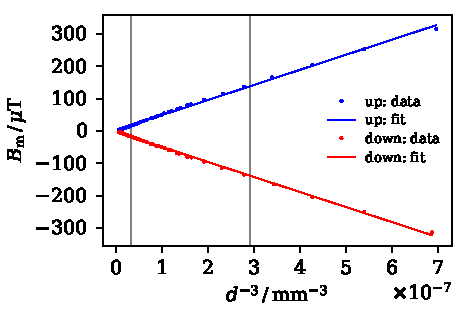
\includegraphics[width=0.75\textwidth]{loss/magnet_array_field_vs_distance.pdf}
\caption[The measured magnetic field of the magnet array versus distance along its center axis.]
{The measured magnetic field of the magnet array versus distance along its center axis.
The fit is acceptable over the range of distances used in the experiment, shown by the vertical gray lines.
The labels refer to the orientation of the field produced by the array.}
\label{fig:magnet_array_field_vs_distance}
\end{figure}

We created a magnetic field normal to the KIDs using an array of seven small NdFeB permanent magnets mounted outside the cryostat.
The magnets were arranged in a triangular lattice \SI{70}{mm} in diameter in order to produce an approximately uniform field at the detector array, which is \SI{28}{mm} by \SI{13}{mm}.
The lateral variation in the field was measured to be less than 10\%. 
As shown in Figure~\ref{fig:magnet_array_field_vs_distance}, the normal component of the magnet array field $\bfield_\magnetarray(\distance)$ was measured as a function of distance $\distance$ from the plane of the magnets along the center axis.
In both orientations, the data were fit to the model
\begin{equation}
\bfield_\magnetarray(\distance)
  =
  a \distance^{-3} + b,
\label{eqn:magnet_array_field_vs_distance}
\end{equation}
as expected for the on-axis field of a dipole plus a possible offset.
The offsets resulting from the fits are a few \si{\micro T}.

To record a data set, we first establish a magnetic field configuration by positioning the magnet array some chosen distance from the KID array.
The cryostat shells are aluminum (well above its $\tc$), the cold stage plate is gold-plated copper, and the other materials near the package are non-magnetic, except where noted below.
Thus, the ambient magnetic field and the field from the permanent magnets should enter the cryostat unaltered.
The total magnetic field that we calculate is
$\bfield(\distance) = \bfield_\ambient + \bfield_\magnetarray(\distance)$,
using the fits of Equation~\ref{eqn:magnet_array_field_vs_distance}.
After setting the field, we cycle the ADR, let the package and KID array cool well below $\tc$, regulate the temperature of the package at $153 \pm \SI{4}{mK}$, then collect data.
For each resonator we first, using a ROACH-based readout, sweep the readout tone frequency across the resonance and fit the data to the resonator model in Equation~\ref{eqn:forwardscattering}, then set the readout tone to the resonance frequency obtained from the fit and collect time-ordered data for \SI{30}{s}.
The data set yields a value for $\qf_\internal$ and a noise spectrum for that magnetic field configuration.
All measurements were recorded using a constant readout tone power of approximately \SI{-100}{dBm} on the feedline, below the onset of nonlinear effects in the resonators.
This process was repeated for a range of distances.
For comparison, we also recorded data with a five-sided mu-metal shield surrounding the cryostat.
The contribution of the ambient field to the interior of the mu-metal shield was measured to be less than \SI{1}{\micro T}, and we take it to be zero when the shield is used.

\subsection{Results}

\begin{figure}[tbp]
\centering
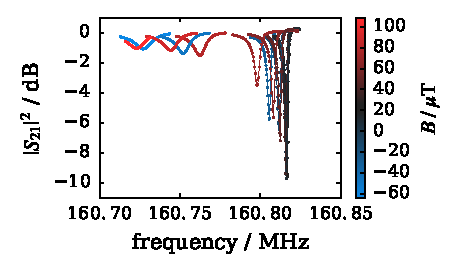
\includegraphics[width=0.75\textwidth]{loss/s21_vs_f_colorbar_B.eps}
\caption
[Forward scattering parameter data at different magnetic fields.]
{The points are forward scattering parameter $\forwardscattering$ data from sweeps of the readout tone across the \SI{161}{MHz} resonance.
The data have been normalized to 1 off-resonance using the fits to the resonator model, which are plotted as lines.
The color bar shows the calculated field $\bfield$ in which the resonator was cooled.}
\label{fig:loss.s21_vs_f}
\end{figure}

Figure~\ref{fig:loss.s21_vs_f} shows the behavior of one resonator as $\bfield_\magnetarray$ is varied.
At higher field magnitudes, $\freadout_\resonator$ and $\qf_\internal$ both decrease, while $\qf_\coupling$ does not change.
As shown in Figure~\ref{fig:loss.iQi_vs_B}, the loss minimum for all three resonators occurs over a range of fields centered near $\bfield = 0$, and the loss increases as the field magnitude departs from this central value.
This result is consistent with previous studies of vortices in thin films, which have generally found that increasing field magnitude creates both higher vortex density in narrow strips and higher loss in resonators.
Direct imaging of the field near narrow strips of thin-film niobium~\autocite{Stan2004PRL} and YBCO~\autocite{Kuit2008PRB} has shown that few or no vortices enter the strip below a threshold field magnitude $\bfield_\threshold$, which varies with the trace width $\tracewidth$ approximately as
$\bfield_\threshold \sim \fluxquantum \tracewidth^{-2}$,
where $\fluxquantum$ is the flux quantum.
Measurements of the vortex-induced loss in aluminum and rhenium thin-film resonators cooled in a magnetic field normal to the film showed that the field had no effect on the loss below a threshold magnitude, and that well above this level the loss was approximately proportional to the excess magnitude above the threshold~\autocite{Song2009PRB}.
The entry of even a single vortex into a region of high current flow in a resonator can cause significant loss~\autocite{Nsanzineza2014PRL}.

\begin{figure}[tb]
\centering
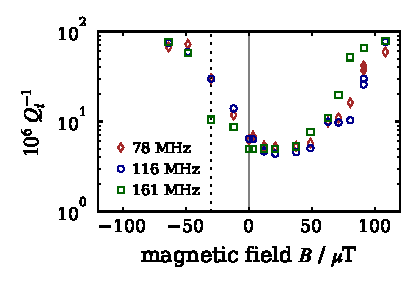
\includegraphics[width=0.7\textwidth]{loss/iQi_vs_B.eps}
\caption
[The inverse internal quality factor of three resonators versus magnetic field.]
{The inverse internal quality factor versus magnetic field ($\bfield_\ambient + \bfield_\magnetarray$), plotted for three resonators.
The vertical gray line marks the field condition when a mu-metal magnetic shield is placed around the cryostat and no magnet array is applied.
The dotted black line marks the field condition with no magnetic shield present and no magnet array.
The points to the left of the dotted black line were recorded with the magnet array polarity reversed so that it augmented the ambient field.
The minimum is likely shifted away from zero because the Heli-Coil inserts in the cold plate of the cryostat can produce a field of about $\SI{25}{\micro T}$.}
\label{fig:loss.iQi_vs_B}
\end{figure}

In Figure~\ref{fig:loss.iQi_vs_B}, the center of the low-loss region is offset from zero by about \SI{25}{\micro T}.
We believe that this offset is caused by fields not included in the calculation of $\bfield$.
First, during the course of these measurements we discovered that the stainless steel Heli-Coil inserts in the millikelvin stage plate are magnetized.
While this Heli-Coil field is not constant across the KID array, its magnitude and direction approximately account for the observed offset.
Second, while the ADR is well-shielded with Vanadium Permendur, it produces a strong field and some leakage is possible.
To estimate the stray field from the ADR, we conducted a separate measurement of the vertical component of the field $\bfield_\ambient + \bfield_\adr$.
Because our Hall probe cannot operate at cryogenic temperatures we made the field measurement \SI{6}{cm} below the package just outside the cryostat.
\todo[inline]{What was the peak field due to the ADR?}
When the current through the ADR magnet is at its peak and the package is at \SI{3}{K}, the ADR field is detectable. % $\bfield_\adr \approx ?$.
However, $\bfield_\adr$ decreases during the ADR cycle because the current in the coil decreases, and the measured field returns to within the measurement uncertainty of $\bfield_\ambient$ when the package reaches \SI{1.4}{K}, indicating that $\bfield_\adr$ is small at the relevant point in the cycle.
Our conclusion is that the ADR field could produce a shift in the center of the low-loss region shown in Figure~\ref{fig:loss.iQi_vs_B}, but it is likely to be a smaller source of systematic error than field from the Heli-Coil inserts.

Interpreting the offset in this way, the threshold field for vortex entry is $\bfield_\threshold \approx \SI{30}{\micro T}$.
As shown in Figure~\ref{fig:loss.experiment}, the widest traces in these resonators are \SI{12}{\micro m}; these are located only where the coupling capacitor runs along part of the much larger capacitor that sets the resonance frequency.
The threshold field for this width is expected to be $\fluxquantum \tracewidth^{-2} = \SI{14}{\micro T}$ (up to a factor that is theoretically expected to be of order unity).
Since these wider traces are near the junction with the inductor, most of the current will flow through them on the way into the \SI{8}{\micro m} wide interdigital capacitor tines, so we expect vortex entry here to produce loss.
Previous measurements of similar lumped-element resonators with a maximum trace width of \SI{8}{\micro m} consistently exhibited high $\qf_\internal$~\autocite{McCarrick2014RSI}.
The crucial difference seems to be that the \SI{12}{\micro m} trace in these devices permits vortex entry at a threshold field less than the ambient field, while the \SI{8}{\micro m} traces did not.

\begin{figure}[tb]
\centering
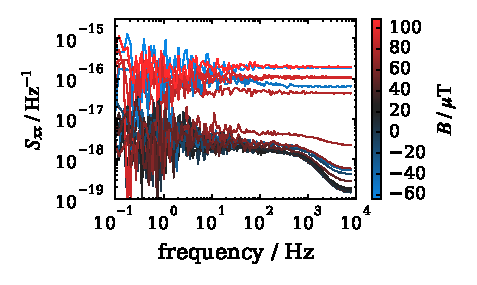
\includegraphics[width=0.75\textwidth]{loss/Sxx_vs_f_colorbar_B.eps}
\caption
[The spectral density of the fractional frequency detuning time series data from one resonator at different magnetic fields.]
{The spectral density of the fractional frequency detuning time series data from the \SI{161}{MHz} resonator.
The color scale corresponds to the magnetic field ($\bfield_\ambient + \bfield_\magnetarray$).
To more clearly show the trend at low frequencies, the lowest 15 harmonics of the \SI{1.412}{Hz} pulse tube cooler frequency have been masked in all of the spectra.
The color bar is the same as Figure~\ref{fig:loss.s21_vs_f}.
}
\label{fig:loss.Sxx_vs_f}
\end{figure}

In SQUIDs, the presence of vortices is known to produce flux noise with a typical $1 / f$ spectral density~\autocite{Dantsker1997APL}.
To investigate the possibility of vortices producing excess noise in the resonators, we decomposed the on-resonance time-ordered data into two real time series corresponding to the fractional frequency shift $\detuning(\time)$ and inverse internal quality factor, or internal loss, $\qf_\internal^{-1}(t)$.
The spectral density $\spectraldensity_{\detuning\detuning}(\faudio)$ of the $\detuning(\time)$ data is shown in Figure~\ref{fig:loss.Sxx_vs_f}.
Larger field magnitudes correspond to higher loss, and thus a higher amplifier noise level.
Besides this expected effect of lower $\qf_\internal$, we see no evidence for additional contributions to the noise due to the presence of vortices.
Only amplifier noise is visible in the internal loss fluctuation spectra (not shown here).

To verify that the superconducting detector package is an effective magnetic shield when cold, we altered the magnetic field after the package had fully cooled and looked for changes in $\qf_\internal$ and $\freadout_\resonator$.
We cooled the package in an initial field condition near the center of the low-loss region in Figure~\ref{fig:loss.iQi_vs_B}, collected the nominal data set, moved the magnet array to establish a new high-field condition at the package, and then collected a second data set.
Between these data sets, neither $\qf_\internal$ nor $\freadout_\resonator$ changed significantly, indicating that the perturbation in the applied magnetic field condition did not affect the resonators either through vortex entry or kinetic inductance non-linearity~\autocite{Healey2008APL,Zmuidzinas2012ARCMP}.
Note that these second points are not shown in Figure~\ref{fig:loss.iQi_vs_B}.
The observation that some vortices remain in the film even when the package is shielding the resonators is consistent with the hysteretic magnetization curves observed in field-cooled type-I thin films~\autocite{Chang1963PL,Miller1964RMP} and with hysteretic loss observed in niobium thin-film resonators~\autocite{Bothner2012PRB}.
We can use a result of \textcite{Stan2004PRL} to estimate the number of vortices $\vortexnumber$ present just below $\tc$ in a trace of width $\tracewidth = \SI{12}{\micro m}$ and length $\tracelength = \SI{1000}{\micro m}$ (this length varies substantially between resonators):
$\vortexnumber
  \approx
  (\bfield - \bfield_\threshold) \tracewidth \tracelength / \fluxquantum
  \sim
  300$
at the highest field magnitudes.

\subsection{Discussion}

When the system is at the operating temperature, the superconducting aluminum package provides some magnetic shielding.
This could be useful for detectors deployed on a telescope, which may be required to move through the Earth's field.
However, our results show that additional shielding is necessary to prevent vortex creation when the module passes through the superconducting transition.
A detector package made from a type-I superconductor with a $\tc$ higher than that of the film should be more effective.

The mu-metal magnetic shield surrounding the cryostat greatly attenuates external fields, but hardware elements such as Heli-Coil inserts or nickel-plated connectors, which are commonly used near the detector package inside the cryostat, could produce magnetic fields strong enough to yield vortices~\autocite{Wang2009APL,Chiaro2016SUST}.

The devices themselves may be modified to reduce vortex formation by adding flux-trapping holes~\autocite{Bothner2011APL,Chiaro2016SUST} or by using a fractal geometry~\autocite{deGraaf2012JAP}.
To cancel the ambient field, it may be more convenient to use a Helmholtz coil instead of permanent magnets~\autocite{Song2009PRB,Mazin2010APL,Bothner2012PRB,Nsanzineza2014PRL}.
Finally, heating the KID arrays inside the superconducting package to the point where the aluminum film becomes normal would cause the vortices to dissipate, and they should not reappear if the package remains superconducting during this process.
